% -*- coding: utf-8 -*-

\chapter{EKF para medidas de distancia}

En el caso de utilizar solamente medidas de distancia a los puntos del mapa, sin que se conozca su orientación respecto a la posición del robot, la ecuación de medida del EKF es unidimensional en lugar de tener dos componentes:
\begin{equation}\label{eq:medida1}
    h_{ij}=\sqrt{(x_{R}-x_{lj})^{2} + (y_{R}-y_{lj})^{2}} - d_{i} = 0,
\end{equation}
donde $d_{i}$ es cada medida de distancia dada por algún sensor estereoceptivo. Se omiten nuevamente los subíndices correspondientes al número de iteración para simplificar la notación.

De este modo, las matrices $H_{x_{ij}}$ y $H_{z_{ij}}$ quedan:
\begin{eqnarray*}
  H_{x_{ij}} & =  & \left [ \frac{x-x_{lj}}{\sqrt{(x-x_{lj})^{2}}}, \frac{y - y_{lj}}{\sqrt{(y - y_{lj})^{2}}},
   0 \right ] ^{T}\\
  H_{z_{ij}} & = & -1
\end{eqnarray*}

La covarianza de una innovación individual quedará:
\begin{equation}\label{eq:s}
    s_{ij}= H_{x_{ij}}^{T}\tilde{P}H_{x_{ij}} + H_{z_{ij}}^{2} \sigma_{d}^{2}
\end{equation}
con $ \sigma_{d}^{2}$ como varianza en las medidas de distancia. Puede apreciarse que la dimensión de este producto es 1. De este modo, las asociaciones se realizarán minimizando la distancia de Mahalannobis, que en este caso resulta ser $\frac{h_{ij}^{2}}{s}$.

La matriz $h$ estará formada por aquellos valores de $h_{ij}$ que hayan minimizado esa distancia para cada observación. Si el número de observaciones asociadas es $t$, tendrá dimensiones ($t\times 1$). La matriz $H_{x}$ tendrá como filas las matrices $H_{x_{i}}$ correspondientes a cada asociación realizada. Sus dimensiones serán ($t\times 3$). La matriz $H_{z}$ será la opuesta de la matriz identidad de dimensión ($t\times t$). La matriz $R$ también será diagonal, con elementos iguales a $ \sigma_{d}^{2}$.

Así, la matriz $S$ tendrá dimensiones ($t \times t$) y $K$, ($3 \times t$).

Por último, quedará:
\begin{eqnarray}
 \hat{x} = \tilde{x} - Kh \label{eq:x1} \\
  \hat{P} = (I-KH_{x})\tilde{P} \label{eq:P1}
\end{eqnarray}

Estas ecuaciones fueron implementadas en Matlab sobre una base de código elaborado por Diego Rodríguez-Losada para ver los resultados proporcionados en la localización del robot a partir de un fichero con datos de observaciones. En la figura \ref{fg:matlab1} se muestra en color verde la trayectoria odométrica correspondiente a un movimiento circular teórico (mostrado en color azul). En rojo se representa la trayectoria corregida mediante esta aplicación del EKF. Puede verse que la información proporcionada por la distancia a los puntos resulta insuficiente para corregir los errores acumulados por la odometría y, al cabo de un cierto tiempo, el robot terminaría perdido.

\begin{figure}[bh]
  % Requires \usepackage{graphicx}
  \centering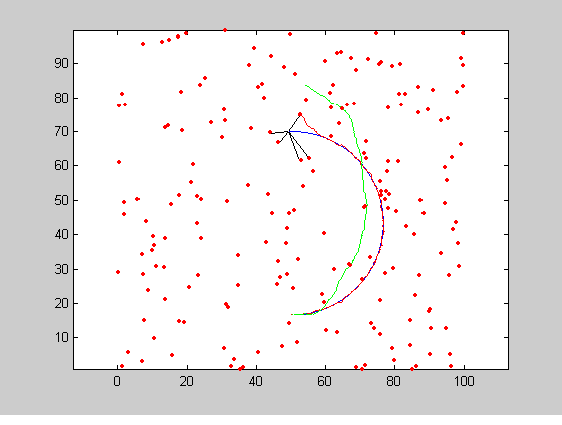
\includegraphics[width=0.5\textwidth]{kalman}
  
  \vspace{0.5cm}
  
  \centering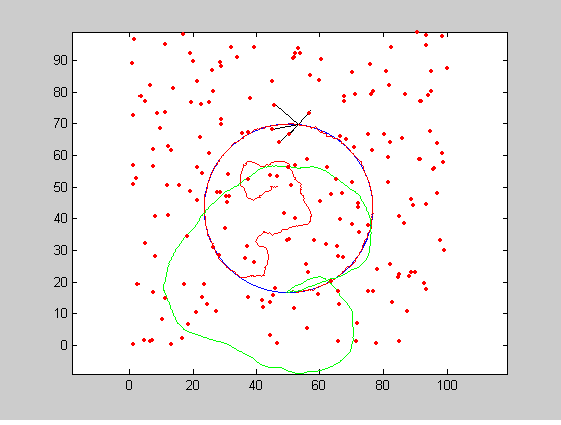
\includegraphics[width=0.5\textwidth]{kalman1}
  \caption{Corrección de la posición en un movimiento circular uniforme mediante medidas de distancia a las observaciones}\label{fg:matlab1}
\end{figure}

Con la información completa de las coordenadas de los puntos observados la asociación de datos se realiza correctamente y esto no sucede, como se puede apreciar en la figura \ref{fg:matlab2}. Se concluye por este motivo que no resulta conveniente utilizar la simplificación desarrollada aquí, aunque podría haber sido de utilidad y, en cualquier caso, sirvió para asentar conocimientos sobre el EKF.

\begin{figure}[h]
  % Requires \usepackage{graphicx}
  \centering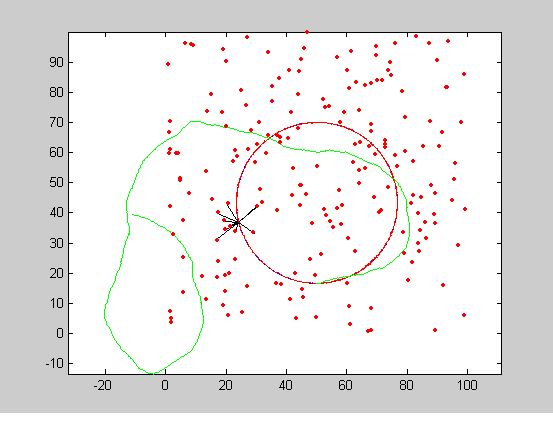
\includegraphics[width=0.5\textwidth]{kalman2}\\
  \caption{Corrección de la posición en un movimiento circular uniforme mediante las coordenadas de las observaciones}\label{fg:matlab2}
\end{figure} 